\documentclass{article}
\usepackage{amsmath}
\usepackage[a4paper,margin=0.7 in,footskip=0.25in]{geometry}
\linespread{1}
\usepackage{caption}
\usepackage{fullpage}
\usepackage{booktabs}
\usepackage{array}
\usepackage{listings}
\usepackage{multicol}
\usepackage{enumerate}
\usepackage{caption}
\usepackage{color}
\usepackage{amssymb}
\lstset{breaklines=true} 
\usepackage{mathrsfs}
\usepackage{dcolumn}

\usepackage{varioref}
\usepackage{float}

\usepackage{graphicx}
% Surround parts of graphics with box
\usepackage{boxedminipage}
% Package for including code in the document
\usepackage{listings}
\usepackage[export]{adjustbox}

\newcommand{\var}[1]{{\ttfamily#1}}% variable
% This is now the recommended way for checking for PDFLaTeX:
\usepackage{ifpdf}
\usepackage{multirow}
\usepackage{hyperref}
\usepackage[utf8]{inputenc}
\usepackage{xparse}
\usepackage[T1]{fontenc}
\setlength{\parindent}{1.5cm}

\usepackage{subcaption}
\renewcommand{\arraystretch}{.2}
\renewcommand{\baselinestretch}{1.2}   % changes \baselineskip to 1.2 x \baselineskip
\renewcommand{\topfraction}{0.9}

\usepackage{setspace}
\usepackage{bm}

\usepackage{array}
\newcolumntype{P}[1]{>{\centering\arraybackslash}p{#1}}
\newcolumntype{M}[1]{>{\centering\arraybackslash}m{#1}}

\pagenumbering{gobble}



\begin{document}

\subsection*{Automated analysis of mission statements to group arts organisations by their activity focus and communities served}

\vspace{.2cm}

\subsubsection*{Methods to learn and understand particularities of plain text data without human help}

\begin{center}
\rule{5cm}{0.4pt}
\end{center}

\noindent
This project was developed using data gathered from \url{http://artbridges.ca/community/community_map}. The dataset contains a small number of mission statements submitted by community art centers in Canada, as well as the associated target community served. To increase the size of the original dataset, data on international community art centers were also collected from \url{https://www.icasc.ca/directory}.

\vspace{.5cm}

\noindent
\textbf{Two Goals:} Automatically group arts community centers into semantically similar categories and find the target clientele for each establishment based on their mission statement.\\

\noindent
\textbf{Limitations:}\\
\noindent
This task is challenging primarily due to the small number of statements. Modern language processing techniques require a lot of data to capture semantic idiosyncrasies. We addressed this problem by introducing additional data - with a modest number of domain-specific texts, combined with a large amount of generic text. Automatic assignment of target clientele is not sensible due to the way the data was entered - a limited number of specific, non-overlapping categories would be ideal. Instead, we built a model to associate different texts together, matching the type of clientele with each mission statement.\\

\noindent
\textbf{Grouping Arts Centers:} One challenge is to determine the ideal number of categories. Four categories consistently yielded the best results. This number could be increased with additional data. Below is a sample of keywords selected in each category. Note that some categories share keywords, as meaning differs depending on context.

\vspace{.8cm}

\begin{table}[H]
\centering
\renewcommand{\arraystretch}{1}
\caption*{Four Topics Automatically Distributed From the ASC Dataset}

\begin{tabular}{| p{1.5cm}|| p{2cm} | p{2cm} | p{2cm} | p{2cm} |}
\hline
      Topics & Work & Performance Arts & Education & Social Issues\\
\hline \hline
          & program & theatre & educate& awareness \\
          & work & dance & youth& world \\
          & workshop  & creativity & young people& politics \\
 Keywords & project  & performance & opportunity& HIV \\
          & participate  & audience & public& women \\
          & collaboration  & story & develop& support \\
          & experience  & express & mission& space \\


\hline 
\end{tabular}
\renewcommand{\arraystretch}{1}
\label{tab:R}
\end{table}

\vspace{.8cm}

\noindent
\textbf{Categorizing Clientele:} The model was able to detect words related to the target clientele. This is a good starting point to classify the arts centers by community served without human help. The plots below are a small sample of randomly selected words and phrases. The different colours represent the machine understanding of semantic groups in the text. 

\vspace{1cm}

\begin{table}[H]
\centering
\renewcommand{\arraystretch}{1.2}
\begin{tabular}{| P{1.6cm}|| P{10cm}|}

\hline
Target & Important words \\
Clientele &              \\
\hline \hline
homeless   & low income, margin, shelter, disadvantaged, poverty, exclusion, gang, addict, violence, disengagement, risk\\
\hline
aboriginal & justice, tolerance, policymaking, empowerment, healing, awakening, change, manifestation, courage \\
\hline
senior     & older adult, health care, dementia, well-being, raise awareness, alumni, concern, finish, difficult, maintain\\
\hline
ex-prisoner& at-risk, youth-at-risk, life skills, urban aboriginal, short-term, under-served, target, men\\



\hline 
\end{tabular}
\renewcommand{\arraystretch}{1}
\caption*{Sample of Automatic Assignment of Keywords to Clientele Type}
\label{tab:group}
\end{table}

\begin{center}
\rule{5cm}{0.4pt}
\end{center}

\begin{figure}[htb!]
\centering
\makebox[0pt][c]{%
\begin{minipage}[b]{0.6\linewidth}
\centering
  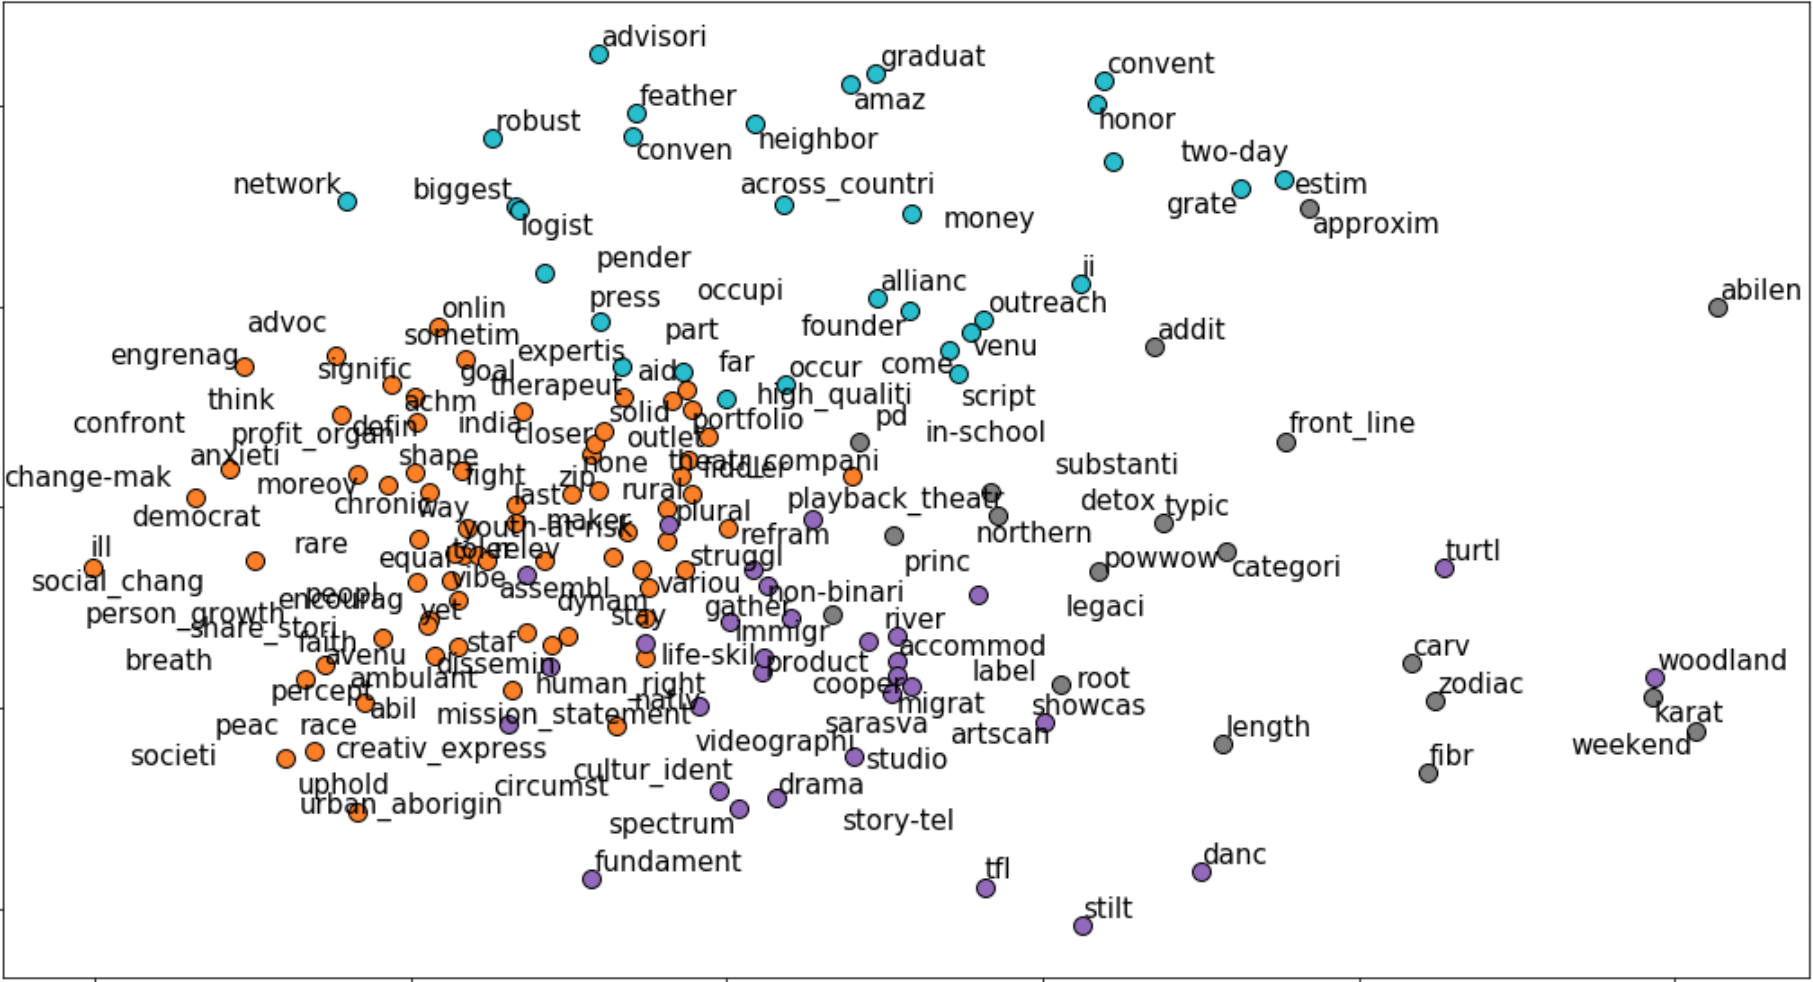
\includegraphics[scale=0.28]{images/word2vecplot}
  \caption*{Automatic Grouping of Word Samples}
\end{minipage}%

\begin{minipage}[b]{0.6\linewidth}
\centering
  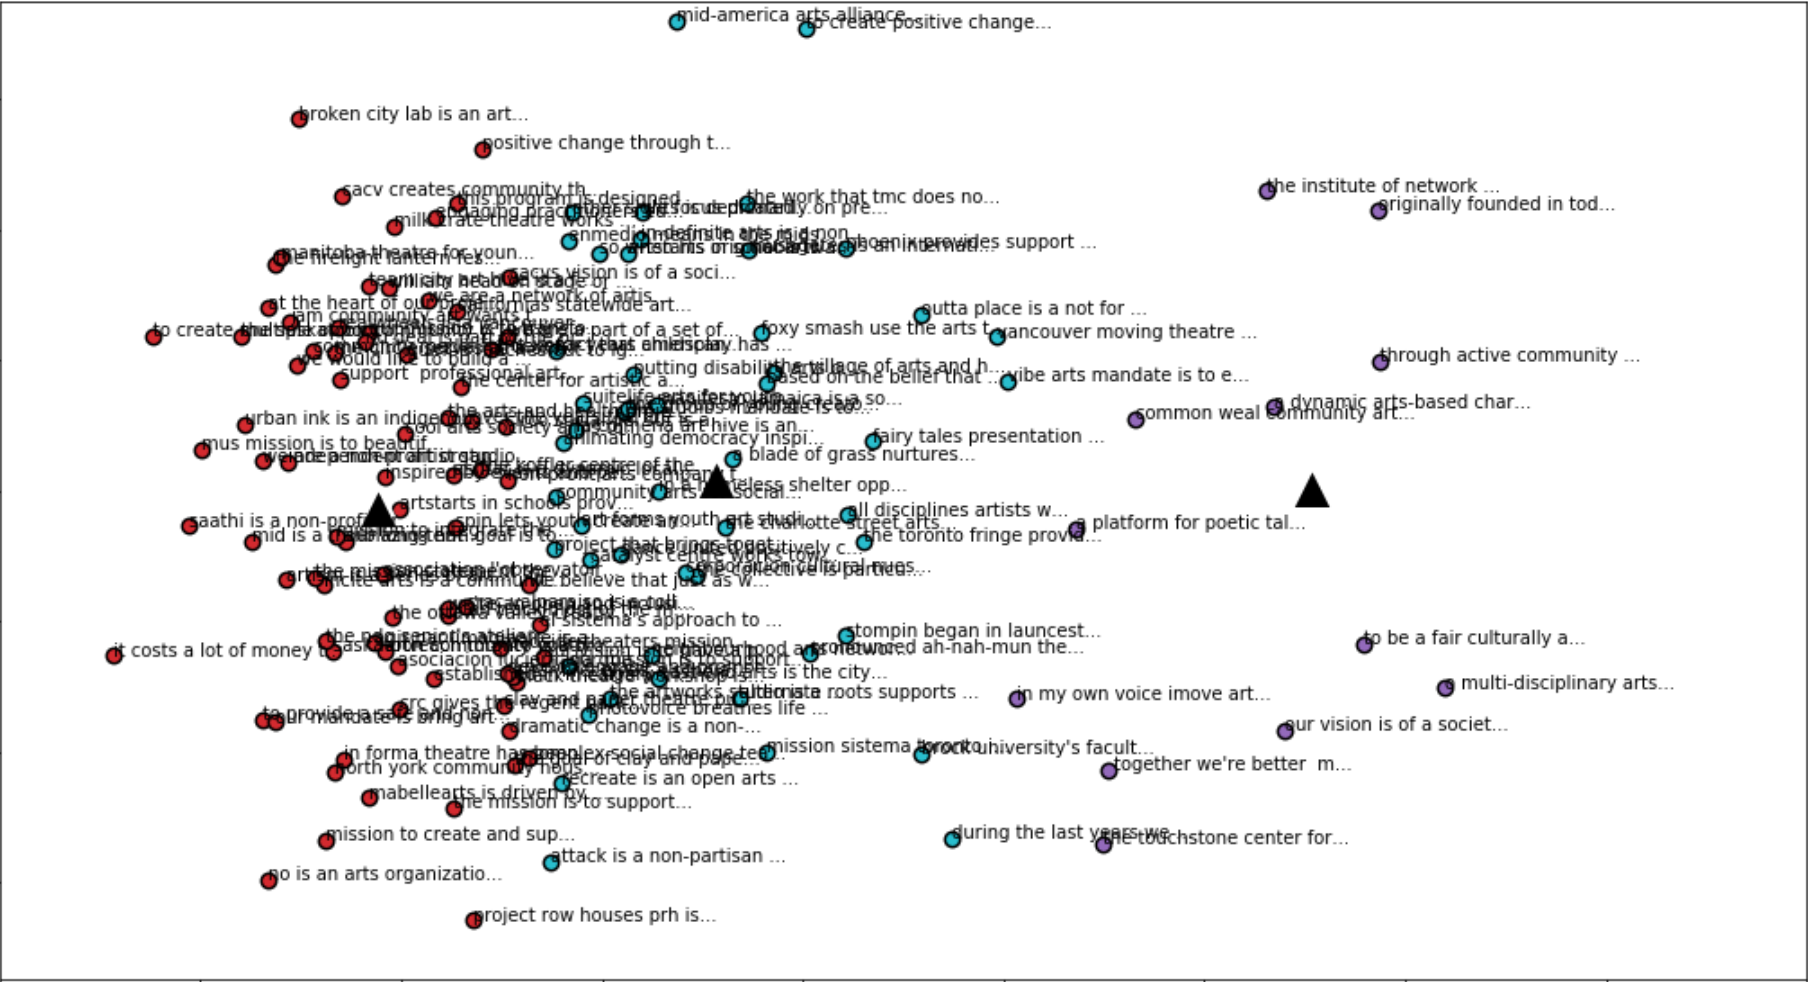
\includegraphics[scale=0.28]{images/doc2vecplot}
  \caption*{Automatic Grouping of Mission Statement Samples}
\end{minipage}%
}%
\end{figure}

\begin{center}
\rule{5cm}{0.4pt}
\end{center}


\noindent
Given the clear identification of meaningful groups based on the small ASC dataset in these preliminary results, automatic grouping and clientele identification appears to be a promising future endeavor. We are looking into expanding on this work and developing further applications. Please contact the authors at SFU KEY for any questions or interest in future collaboration.

\vspace{1.2cm}

\small{
\noindent
\underline{Contact Information}:\\
Dr. Steven Bergner: \texttt{steven\_bergner@sfu.ca}\\
Maude Lachaine: \texttt{mlachain@sfu.ca}\\
\noindent
KEY, Simon Fraser University\\
Spring 2019
}\\

\begin{figure}
    \adjustimage{width=.6\textwidth, center}{images/keylogo}
\end{figure}

\end{document}